\documentclass{article}\usepackage[]{graphicx}\usepackage[]{xcolor}
% maxwidth is the original width if it is less than linewidth
% otherwise use linewidth (to make sure the graphics do not exceed the margin)
\makeatletter
\def\maxwidth{ %
  \ifdim\Gin@nat@width>\linewidth
    \linewidth
  \else
    \Gin@nat@width
  \fi
}
\makeatother

\definecolor{fgcolor}{rgb}{0.345, 0.345, 0.345}
\newcommand{\hlnum}[1]{\textcolor[rgb]{0.686,0.059,0.569}{#1}}%
\newcommand{\hlsng}[1]{\textcolor[rgb]{0.192,0.494,0.8}{#1}}%
\newcommand{\hlcom}[1]{\textcolor[rgb]{0.678,0.584,0.686}{\textit{#1}}}%
\newcommand{\hlopt}[1]{\textcolor[rgb]{0,0,0}{#1}}%
\newcommand{\hldef}[1]{\textcolor[rgb]{0.345,0.345,0.345}{#1}}%
\newcommand{\hlkwa}[1]{\textcolor[rgb]{0.161,0.373,0.58}{\textbf{#1}}}%
\newcommand{\hlkwb}[1]{\textcolor[rgb]{0.69,0.353,0.396}{#1}}%
\newcommand{\hlkwc}[1]{\textcolor[rgb]{0.333,0.667,0.333}{#1}}%
\newcommand{\hlkwd}[1]{\textcolor[rgb]{0.737,0.353,0.396}{\textbf{#1}}}%
\let\hlipl\hlkwb

\usepackage{framed}
\makeatletter
\newenvironment{kframe}{%
 \def\at@end@of@kframe{}%
 \ifinner\ifhmode%
  \def\at@end@of@kframe{\end{minipage}}%
  \begin{minipage}{\columnwidth}%
 \fi\fi%
 \def\FrameCommand##1{\hskip\@totalleftmargin \hskip-\fboxsep
 \colorbox{shadecolor}{##1}\hskip-\fboxsep
     % There is no \\@totalrightmargin, so:
     \hskip-\linewidth \hskip-\@totalleftmargin \hskip\columnwidth}%
 \MakeFramed {\advance\hsize-\width
   \@totalleftmargin\z@ \linewidth\hsize
   \@setminipage}}%
 {\par\unskip\endMakeFramed%
 \at@end@of@kframe}
\makeatother

\definecolor{shadecolor}{rgb}{.97, .97, .97}
\definecolor{messagecolor}{rgb}{0, 0, 0}
\definecolor{warningcolor}{rgb}{1, 0, 1}
\definecolor{errorcolor}{rgb}{1, 0, 0}
\newenvironment{knitrout}{}{} % an empty environment to be redefined in TeX

\usepackage{alltt}
\usepackage{amsmath} %This allows me to use the align functionality.
                     %If you find yourself trying to replicate
                     %something you found online, ensure you're
                     %loading the necessary packages!
\usepackage{amsfonts}%Math font
\usepackage{graphicx}%For including graphics
\usepackage{hyperref}%For Hyperlinks
\usepackage[shortlabels]{enumitem}% For enumerated lists with labels specified
                                  % We had to run tlmgr_install("enumitem") in R
\hypersetup{colorlinks = true,citecolor=black} %set citations to have black (not green) color
\usepackage{natbib}        %For the bibliography
\setlength{\bibsep}{0pt plus 0.3ex}
\bibliographystyle{apalike}%For the bibliography
\usepackage[margin=0.50in]{geometry}
\usepackage{float}
\usepackage{multicol}

%fix for figures
\usepackage{caption}
\newenvironment{Figure}
  {\par\medskip\noindent\minipage{\linewidth}}
  {\endminipage\par\medskip}
\IfFileExists{upquote.sty}{\usepackage{upquote}}{}
\begin{document}

\vspace{-1in}
\title{Lab XX -- MATH 240 -- Computational Statistics}

\author{
  Danny Molyneux \\
  Colgate University  \\
  Mathematics  \\
  {\tt dmolyneux@colgate.edu}
}

\date{}

\maketitle

\begin{multicols}{2} \raggedcolumns
%\raggedcolumns % If your spacing gets messed up try uncommenting 
                % this line
\begin{abstract}
In this lab, we are discussing margin of error: what it means, different ways to interpret it, and what variables have an impact on it.
\end{abstract}
\noindent \textbf{Keywords:} Sample size, margin of error, polling, resampling.
\section{Introduction}
In this lab, we are going to test some of Gallup's claims, including the one about the margin of error halving if we increase sample size from 1000 to 2000. To do this we will have to assume the population proportion.

We can also gather information without making an assumption about the population proportion, and that is through the method of resampling. We can take the data from Gallup's survery given the fact that we know the results he gathered, and we can perform many resamples (10000).

Lastly, if we want to see what factors impact margin of error (MOE) rather than just the sample size, we can plot it as a function of both sample size and sample proportion. We can do the same but while calculating the Wilson MOE, to see if we gain any additional insights.

\section{Methods}
The only data we are really working with here is Gallup's survey data from February 2025. We know that the sample size is 1004 adults living in all 50 states of the U.S, and that 39\% were satisfied with the position of the U.S. today, while 59\% were dissatisfied (2\% had no opinion). Gallup also reported that the margin of error was 4\%, but it's not clear how much he rounded that by.

So like I said before, we can approximate the sampling distribution for p without assuming the actual population proportion is 0.39. Instead, we can replicate Gallup's data by making a vector with 1004 data points, and making 39\% of the data a "1" (satisfied), and the rest of the data a "0" (dissatisfied or no opinion). This is technically not perfectly accurate because I am treating dissatisfied and no opinion equally, but when we are only studying the satisfied proportion, it is okay to treat them equally. With this data, we can perform resampling many times (10000), by using the \texttt{sample()} method from the base \texttt{R} package.

I also said that I want to test Gallup's statement about how the MOE changes when doubling the population from 1000 to 2000. We can do this by using the \texttt{rbinom()} function, and then using the \texttt{ggplot2} \citep{ggplot2} and \texttt{tidyverse} \citep{tidyverse} packages to plot the density of the sample proportions for both populations.

Lastly, in order to see MOE's relationship with both sample size (n) and proportion (p), we can again use \texttt{rbinom()} to simulate the data, and \texttt{quantile()} to calculate the range and eventually the MOE. Now that we have two independent variables, we can use \texttt{geom\textunderscore raster()}. This will make a plot that is easy to visualize the MOE's relationship with both variables.
\section{Results}
Below are the histograms of 10000 polls with sample size 1004, and then with sample size 2008 (doubled).

\begin{Figure}
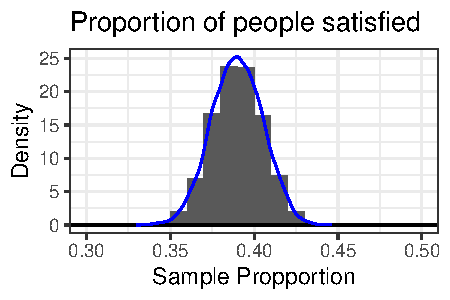
\includegraphics{Histogram1.pdf}
\captionof{figure}{10000 polls with n=1004, p= 0.39}
\label{fig:histogram1}
\end{Figure}

\begin{Figure}
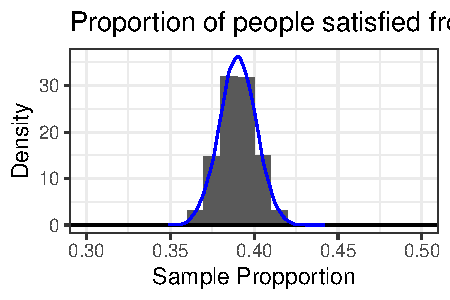
\includegraphics{Histogram2.pdf}
\captionof{figure}{10000 polls with n=2008, p= 0.39}
\label{fig:histogram2}
\end{Figure}

You can see that the plots are different, but they do both follow a relatively normal distribution. This is because the samples are random, and the sample sizes are well over 30. One thing you can't see from the graphs are the margins of error. After calculating them, I got an MOE of 0.03037845 (approx 3\%) for figure \ref{fig:histogram1}, and an MOE of 0.02141435 (approx 2\%) for figure \ref{fig:histogram2}. So although they line up pretty well for the 2008 sample size, the MOE was not halved. It's hard to know how different my MOE is from Gallup's for the original sample size because we don't know how much he rounded by, but there is definitely a difference.

Now let's look at the sampling distribution for p from using the resampling method. 

\begin{Figure}
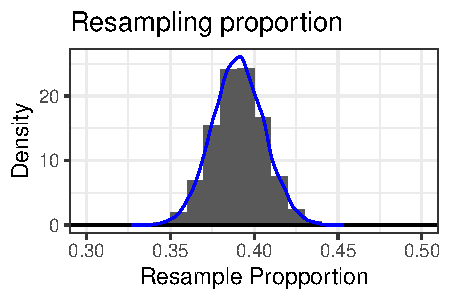
\includegraphics{Resampling.pdf}
\captionof{figure}{Resampling sample proportion} 
\label{fig:resampling}
\end{Figure}
We can see again that it follows a relatively normal distribution for the same reasons as before. For this distribution, I calculated an MOE of 0.03087649 (approx 3\%). This is very similar to the MOE from before when using a sample size of 1004. So our resampling method was successfull in giving us a very similar distribution to the real data, without making any assumptions about the population proportion.

Finally, let's look at \texttt{geom\textunderscore raster()} plots of the MOE, with respect to sample size and proportion.

\begin{Figure}
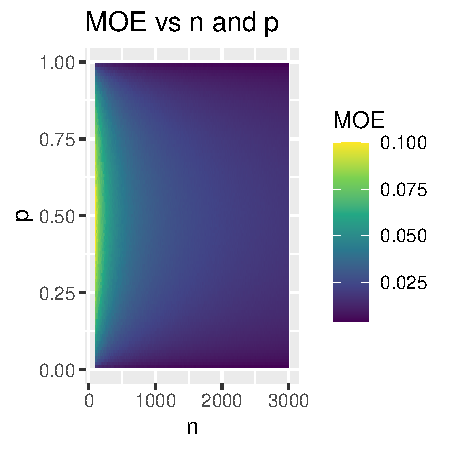
\includegraphics{MOE.pdf}
\captionof{figure}{MOE vs. n and p} 
\label{fig:MOE}
\end{Figure}

\begin{Figure}
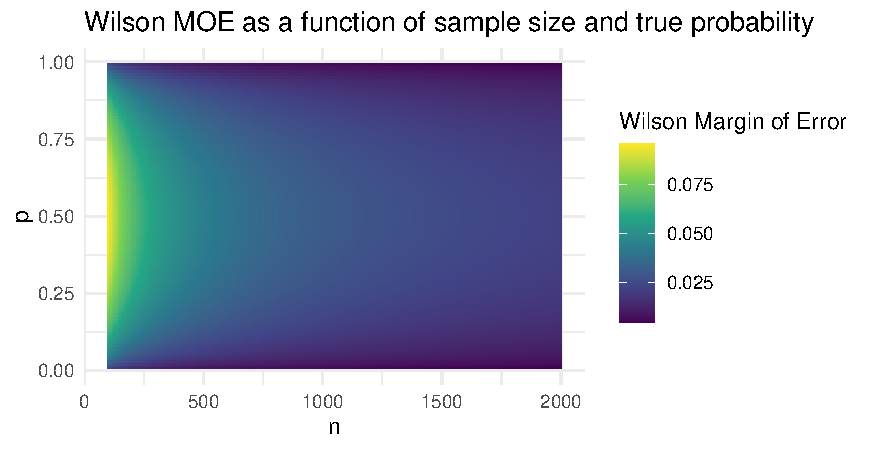
\includegraphics{Wilson.plot.pdf}
\captionof{figure}{Wilson MOE vs. n and p} 
\label{fig:Wilson}
\end{Figure}
Figure \ref{fig:MOE} is the estimated margin of error, and Figure \ref{fig:Wilson} is the estimated Wilson margin of error. As you can see, the MOE on both plots definitely decreases as sample size increases. However, sample proportion p definitely has influence as well. When p is near 0 or 1, the MOE is small even when n is small. This is because the p(1-p) in the MOE formula is very small if p is near 0 or 1, resulting in the entire formula resulting in a small value. You can see based on the color that when p is near 0 or 1, and n is big, the MOE gets even lower than 2\%
\section{Discussion}
Obviously someone conducting public opinion polls can't control what the sample proportion is going to be, but they should keep in mind that if the proportion is not going to be anywhere near 0 or 1, they will need a larger sample size in order to get a small MOE. So for Gallup, 0.39 is a pretty centered proportion, so 1004 may not be quite large enough of a sample size if the goal is to get a very small margin of error.

An important question is: Is it worth it to double the cost, in order to go from a 4\% MOE to a 2\% MOE? And based on my calulations, it was actually from a 3\% MOE to a 2\% MOE, meaning it decreased by 33\%. obviously it depends on the budget of the pollster, and the goal for the MOE. However, I think for big companies it is typically worth the extra money, because having the most accurate and precise polls is how to become the most credible and popular source.

%%%%%%%%%%%%%%%%%%%%%%%%%%%%%%%%%%%%%%%%%%%%%%%%%%%%%%%%%%%%%%%%%%%%%%%%%%%%%%%%
% Bibliography
%%%%%%%%%%%%%%%%%%%%%%%%%%%%%%%%%%%%%%%%%%%%%%%%%%%%%%%%%%%%%%%%%%%%%%%%%%%%%%%%
\vspace{2em}

\begin{tiny}
\bibliography{bibliography}
\end{tiny}
\end{multicols}


\end{document}
